\documentclass[11pt]{article}
\usepackage[T1]{fontenc}
\usepackage[margin=1.25in]{geometry}
\usepackage[expansion=false]{microtype}
\usepackage{amsmath,amssymb}
\usepackage{booktabs,tabularx,array}
\usepackage{enumitem}
\usepackage{xcolor}
\usepackage{tikz}
\usetikzlibrary{positioning,calc,matrix,fit,backgrounds}
\usepackage{hyperref}
\emergencystretch=3em
\setlength{\parskip}{0.55em}
\setlength{\parindent}{0pt}

\definecolor{stands}{RGB}{214,232,247}
\definecolor{defeated}{RGB}{222,222,222}
\definecolor{unres}{RGB}{252,238,190}
\definecolor{ink}{RGB}{40,40,40}

% numbered marker used in the figure and in the text
\newcommand{\hd}[1]{{\scriptsize\bfseries\scshape #1}}
\newcommand{\mk}[1]{\textcircled{\scriptsize\bfseries #1}}

\title{Reader's Guide to a Claim Page}
\author{Flyxion\\\small Independent Researcher}
\date{30 September 2026}

\begin{document}
\maketitle

\begin{abstract}
\noindent
A claim page in the system described by the monograph \emph{Adversaria: A Specification for a Public Claim Graph} is meant to be read by people who have never seen the mathematics behind it. This guide explains, in plain language, the four ideas a reader needs: the claim, its scope, the objections to it, and its status. It works through one annotated drawing of a claim page, built around an invented claim about roof coverings, and it explains why the page shows a row of separate facts in place of a single score. The page is a drawing made for this guide and not a screenshot. No real interface is described, no reader was tested, and nothing here shows that readers will find the layout easier than another. The formal statements behind the page are proved in the monograph; the guide states them in words.
\end{abstract}

\section{Who this guide is for}

Most people who meet a disputed question online meet it as a page of prose, or as a single figure beside a name. A claim page is a third thing. It is a place where one claim, the region it is asserted over, the evidence offered, the challenges raised and the present state of play are laid out together, so that a reader can see where the claim stands and where it does not.

This guide is for a reader who arrives at such a page for the first time. It assumes no mathematics and no vocabulary. It introduces seven words, all of them in ordinary use: claim, scope, grounds, warrant, objection, reply and status. Each gets a plain-language version first and a precise one second. After that comes a drawing of a page with its parts numbered, a short routine for reading it, and a list of things the page does not tell you.

A caution belongs at the start. The page in the drawing is invented, and so is its subject. Nothing in it reports a finding about roofs or about anything else. The drawing is a teaching device. A real page may arrange the same facts differently.

\section{Four ideas in plain language}\label{sec:words}

\begin{center}
\small
\begin{tabularx}{\textwidth}{@{}l X X@{}}
\toprule
word & in plain language & a little more precisely\\
\midrule
claim & One definite statement, with its key words pinned down, and a note on what kind of statement it is (a description, a cause, a mechanism, a recommendation, a guess). & A kernel (the exact statement and the meaning of each term that needs one) together with a scope and a stated kind of assertion.\\
scope & The places, people, periods and conditions where the claim is being asserted. Outside the scope the claim says nothing. & A region of a space of units described by coordinates such as population, context, time and measurement method.\\
objection & A reasoned challenge that says what it is aimed at and where it applies. It is itself an argument and can be answered. & An argument whose conclusion denies the claim, a piece of its evidence, or the rule connecting evidence to claim, over a stated region.\\
status & What can be said right now about how the claim is doing, given the records and a named way of weighing them. It is worked out fresh each time and is never a verdict written in by hand. & A field over the scope: at each unit a labeled outcome (stands, defeated, unresolved) and a vector of separate components.\\
\bottomrule
\end{tabularx}
\end{center}

Two further words complete the picture. \emph{Grounds} are the evidence offered: measurements, records, documents, each with an account of where it came from. A \emph{warrant} is the stated rule that lets the grounds support the claim: for example, that matched comparisons with random assignment support a claim about a difference in temperature on the kinds of roof studied. A page that shows the warrant lets a reader ask whether the evidence was good and, separately, whether the step from evidence to claim was good.

\section{An annotated page}\label{sec:page}

Figure~\ref{fig:page} is a drawing of a claim page for an invented claim: that a moss mat on a roof lowers attic temperature by at least two degrees on hot days. The numbered markers are explained after the figure. Every number on the drawing is invented.

\begin{figure}[!p]
\centering
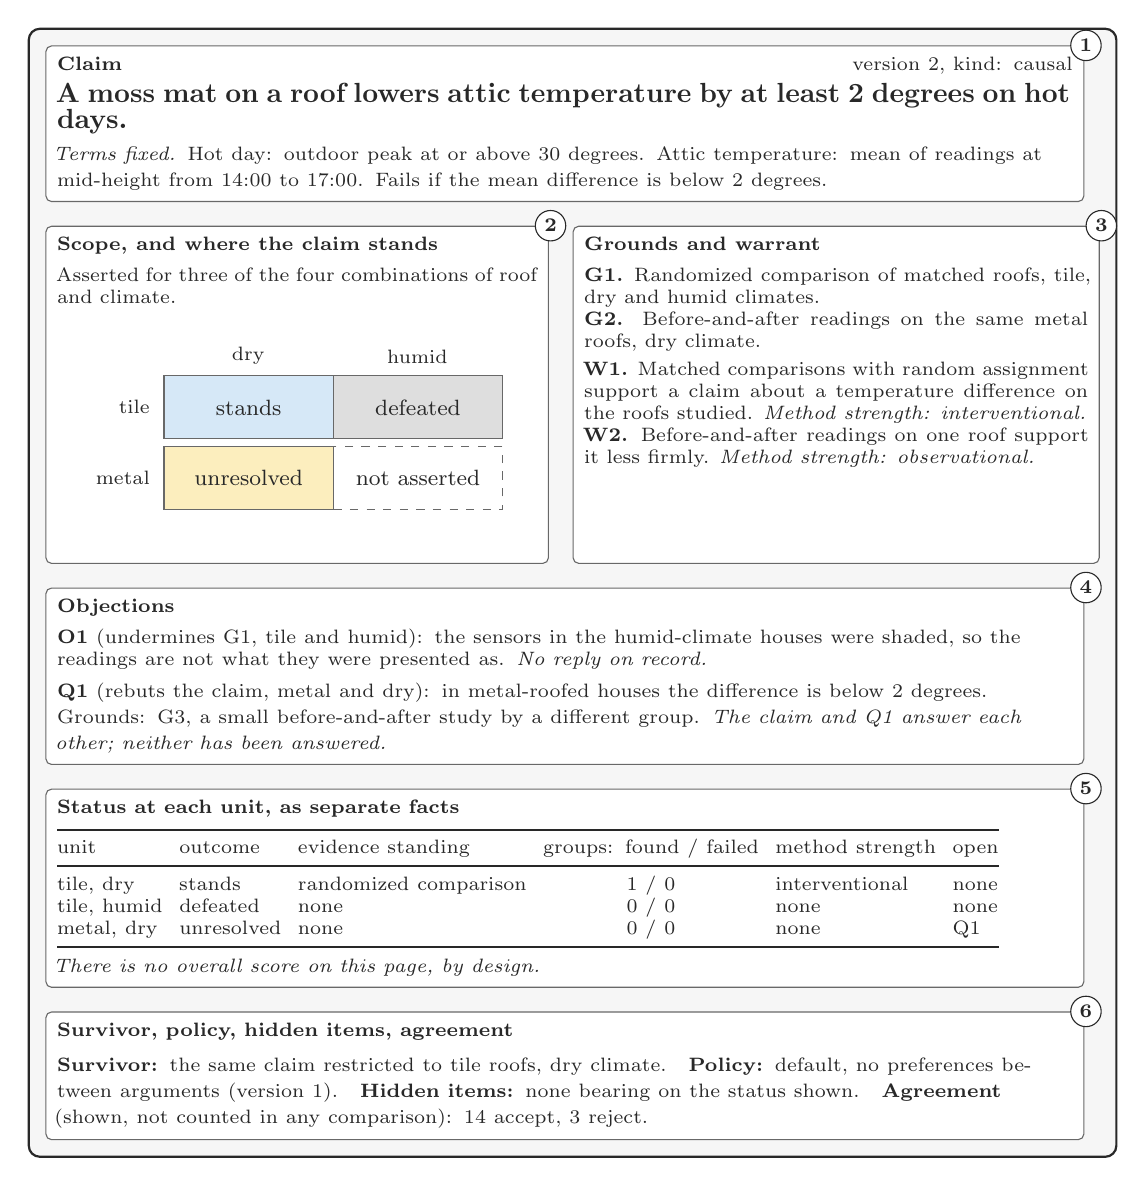
\begin{tikzpicture}[
  font=\footnotesize, every node/.style={text=ink},
  box/.style={draw=ink!70, rounded corners=2pt, inner sep=4pt, align=left, fill=white, anchor=north west},
  tag/.style={circle, draw=ink, fill=white, inner sep=0.8pt, font=\scriptsize\bfseries, minimum size=11pt},
  cell/.style={draw=ink!70, minimum width=2.15cm, minimum height=0.8cm, align=center, inner sep=2pt}
]
\node[box, text width=12.9cm] (claim) at (0,0)
 {\hd{Claim}\hfill {\scriptsize version 2, kind: causal}\\[2pt]
  {\normalsize\textbf{A moss mat on a roof lowers attic temperature by at least 2 degrees on hot days.}}\\[2pt]
  \scriptsize\emph{Terms fixed.} Hot day: outdoor peak at or above 30 degrees. Attic temperature: mean of readings at mid-height from 14:00 to 17:00. Fails if the mean difference is below 2 degrees.};
\node[box] (scope) at ([yshift=-3mm]claim.south west) {\begin{minipage}[t][4.0cm][t]{6.1cm}\hd{Scope, and where the claim stands}\\[3pt]
 \scriptsize Asserted for three of the four combinations of roof and climate.\end{minipage}};
\begin{scope}[shift={(scope.north west)}]
 \node[cell, fill=stands, anchor=north west] at (1.5,-1.9) {stands};
 \node[cell, fill=defeated, anchor=north west] at (3.65,-1.9) {defeated};
 \node[cell, fill=unres, anchor=north west] at (1.5,-2.8) {unresolved};
 \node[cell, dashed, anchor=north west] at (3.65,-2.8) {not asserted};
 \node[font=\scriptsize, anchor=east] at (1.45,-2.3) {tile};
 \node[font=\scriptsize, anchor=east] at (1.45,-3.2) {metal};
 \node[font=\scriptsize, anchor=south] at (2.575,-1.88) {dry};
 \node[font=\scriptsize, anchor=south] at (4.725,-1.88) {humid};
\end{scope}
\node[box] (grounds) at ([xshift=3mm]scope.north east) {\begin{minipage}[t][4.0cm][t]{6.4cm}\hd{Grounds and warrant}\\[3pt]
 \scriptsize\textbf{G1.} Randomized comparison of matched roofs, tile, dry and humid climates.\\
 \textbf{G2.} Before-and-after readings on the same metal roofs, dry climate.\\[2pt]
 \textbf{W1.} Matched comparisons with random assignment support a claim about a temperature difference on the roofs studied. \emph{Method strength: interventional.}\\
 \textbf{W2.} Before-and-after readings on one roof support it less firmly. \emph{Method strength: observational.}\end{minipage}};
\node[box, text width=12.9cm] (obj) at ([yshift=-3mm]scope.south west) {\hd{Objections}\\[3pt]
 \scriptsize\textbf{O1} (undermines G1, tile and humid): the sensors in the humid-climate houses were shaded, so the readings are not what they were presented as. \emph{No reply on record.}\\[2pt]
 \textbf{Q1} (rebuts the claim, metal and dry): in metal-roofed houses the difference is below 2 degrees. Grounds: G3, a small before-and-after study by a different group. \emph{The claim and Q1 answer each other; neither has been answered.}};
\node[box, text width=12.9cm] (vec) at ([yshift=-3mm]obj.south west) {\hd{Status at each unit, as separate facts}\\[3pt]
 \scriptsize\setlength{\tabcolsep}{3pt}
 \begin{tabular}{@{}l l l c l l@{}}
 \toprule
 unit & outcome & evidence standing & groups: found / failed & method strength & open\\
 \midrule
 tile, dry & stands & randomized comparison & 1 / 0 & interventional & none\\
 tile, humid & defeated & none & 0 / 0 & none & none\\
 metal, dry & unresolved & none & 0 / 0 & none & Q1\\
 \bottomrule
 \end{tabular}\\[3pt]
 \emph{There is no overall score on this page, by design.}};
\node[box, text width=12.9cm] (foot) at ([yshift=-3mm]vec.south west) {\hd{Survivor, policy, hidden items, agreement}\\[3pt]
 \scriptsize\textbf{Survivor:} the same claim restricted to tile roofs, dry climate.\quad
 \textbf{Policy:} default, no preferences between arguments (version 1).\quad
 \textbf{Hidden items:} none bearing on the status shown.\quad
 \textbf{Agreement} (shown, not counted in any comparison): 14 accept, 3 reject.};
\node[tag] at ([shift={(0.02,0.0)}]claim.north east) {1};
\node[tag] at ([shift={(0.02,0.0)}]scope.north east) {2};
\node[tag] at ([shift={(0.02,0.0)}]grounds.north east) {3};
\node[tag] at ([shift={(0.02,0.0)}]obj.north east) {4};
\node[tag] at ([shift={(0.02,0.0)}]vec.north east) {5};
\node[tag] at ([shift={(0.02,0.0)}]foot.north east) {6};
\begin{scope}[on background layer]
 \node[draw=ink, line width=0.8pt, rounded corners=4pt, inner sep=6pt, fit=(claim)(scope)(grounds)(obj)(vec)(foot), fill=ink!4] {};
\end{scope}
\end{tikzpicture}
\caption{A drawing of a claim page for an invented claim. Six regions are numbered. All content is invented, and the layout is one of many possible.}\label{fig:page}
\end{figure}

\paragraph{\mk{1} The claim.} The sentence is at the top, with its key terms pinned down underneath and a note on what kind of statement it is. The last line says what it would take for the claim to fail. Read this first. A large share of disputes are quarrels about what a word means, and when the terms are fixed in plain view, a quarrel of that kind shows up as one.

\paragraph{\mk{2} The scope, and where the claim stands.} The grid shows the combinations the claim is asserted for. Here the coordinates are roof type and climate, and three of the four cells belong to the claim. The fourth is dashed because the claim says nothing there. The label in each cell is the outcome at that unit, and the next section explains the three words. The grid also shows something the claim sentence cannot: the claim is asserted over three cells, and its fate is different in each.

\paragraph{\mk{3} The grounds and the warrant.} The evidence offered is listed first, each item with a plain description of how it was collected. The rules that connect the evidence to the claim come next, each with a note on method strength: how well the method can rule out other explanations, from none, through observational, to interventional. A reader who doubts the claim can now ask two separate questions. Was this evidence sound? And does evidence of this kind support a claim of this kind?

\paragraph{\mk{4} The objections.} Each objection says what it is aimed at and where it applies, and whether anyone has answered it. O1 is aimed at a piece of evidence. Q1 is aimed at the conclusion itself, on one cell. The page records who has replied, and it lists objections as well as claims in the place where the claim is displayed.

\paragraph{\mk{5} The status, as separate facts.} One row for each unit of the scope. The columns are the kind of evidence that currently stands, the number of independent groups who found the result and the number who tried and failed to repeat it, the method strength of the best evidence standing, and the challenges still open. There is no total at the bottom. Section~\ref{sec:noscore} says why.

\paragraph{\mk{6} The survivor, the view and the agreement.} The survivor is the largest part of the claim that stands everywhere. The policy line names the rule for weighing conflicting arguments that produced everything above. The line about hidden items says whether any objection bearing on the status was left out of what this reader can see. The agreement counts are shown for information and are kept out of every comparison.

\section{Reading the verdict words}\label{sec:verdicts}

Each cell carries one of three outcomes, and none of them means ``true'' or ``false.''

\begin{itemize}[nosep]
\item \textbf{Stands.} Every challenge aimed at the claim at this unit has itself been answered. It is the outcome for a claim nobody has challenged, and also for one whose challengers have all been answered.
\item \textbf{Defeated.} Some challenge aimed at the claim at this unit stands, meaning that nothing has answered it. Defeat here is the outcome at one unit under one policy. It is not a finding that the claim is false.
\item \textbf{Unresolved.} The claim and a challenge to it answer each other, or are caught in a circle of challenges, and nothing has broken the tie. The page says so and does not pick a winner.
\end{itemize}

Look back at the drawing. On tile roofs in a dry climate the claim stands, because nobody has aimed anything at it there. On tile roofs in a humid climate it is defeated, because O1 is aimed at G1 there, nothing answers O1, and G1 was the only evidence for that unit. On metal roofs in a dry climate the claim is unresolved: Q1 says the opposite over that cell, the claim says its own, and each challenges the other, so neither is ahead. The page does not declare the claim dead because of the two bad cells, and it does not hide them because of the good one.

Two things follow from this design that are worth knowing before reading any page.

\paragraph{An objection stays where it was aimed.} O1 concerns tile roofs in humid houses. It has no effect on tile roofs in dry climates, and the drawing shows none. An objection that names a region can change the outcome only inside that region. This is one of the guarantees proved in the monograph, and it is what lets a page stay readable when many challenges have been filed.

\paragraph{A narrower claim can survive.} The survivor line says that the same claim, restricted to tile roofs in a dry climate, stands throughout. A claim that has been challenged in part is not thrown away. Its largest undefeated part is named, and the part that was removed is shown with the reason.

\section{Three kinds of objection}\label{sec:objections}

The page labels each objection by what it is aimed at, because the labels say what is left standing.

\begin{center}
\small
\begin{tabularx}{\textwidth}{@{}l X X@{}}
\toprule
label on the page & in plain language & what it leaves standing\\
\midrule
undermines a ground & ``This evidence is not what it was presented as.'' & The rule connecting evidence to claim is untouched, so the same rule applied to other evidence can still support the claim.\\
undercuts a warrant & ``Evidence of this kind does not support a claim of this kind here.'' & The evidence is untouched and can still support other claims.\\
rebuts the claim & ``The opposite holds in this region.'' & Both evidence and rule are untouched, and two argued positions now face each other.\\
\bottomrule
\end{tabularx}
\end{center}

In the drawing, O1 undermines a ground and Q1 rebuts the claim. A page with no place for the warrant could not tell a study that was fine and an inference that was not from a study that was not fine. A reader who sees an objection labeled in this way knows what to ask next.

An objection must say where it applies. One that never meets the region of the thing it is aimed at does not count as an objection to it. And an objection is itself an argument that can be answered, which is why the page shows replies.

\section{Why there is no single score}\label{sec:noscore}

The status block has five columns and no total. The reason is worth stating in plain terms, because a total is the first thing many readers look for.

Suppose two claims are being compared. The first rests on a single controlled trial. The second rests on three independent observational studies. On method strength the first is better, because a controlled trial can rule out rival explanations that observational studies cannot. On independent groups the second is better, three against one. Neither is at least as good on every column, so neither comes out ahead without an extra decision: how many independent observational studies are worth one trial. That is a judgment about what counts as good evidence, and communities differ on it.

A single score has to make that decision for every reader, silently, in the act of adding up. The monograph proves the exact sense of this. A score that respects every comparison the record does establish must still put the two claims in some order, or tie them, and the record contains no instruction for which. Weighted sums also have a flaw of their own. A claim that is moderate on every column and beaten by none can fail to come out first under any choice of positive weights, so it disappears from the ranking although nothing beats it.

What a page can offer instead is the row of separate facts and, where a reader wants an order, a view that says what it counts. A ranked list built on such a view names the view, shows the claims that nothing beats, and leaves the order within that set to the view. The exchange rate is in the open, so readers can argue with it.

\section{Five steps for reading a page}\label{sec:steps}

\begin{enumerate}[label=\textbf{\arabic*.}, nosep]
\item Read the claim sentence and the fixed terms \mk{1}. Ask whether you mean the same thing by the key words.
\item Find the cell of the scope grid that matches your case \mk{2}. If your case is outside the scope, the claim says nothing about it.
\item Read the outcome in that cell. Stands, defeated and unresolved each tell you something different about what to do next.
\item Read the objections aimed at that cell \mk{4}, and which part of the argument each one attacks. Check whether anyone has answered them.
\item Read the status row for that cell \mk{5}, and the policy line \mk{6}. Ask whether you would weigh conflicts differently from the named policy. If so, the page can be recomputed under a policy you name, and the difference will be traceable to the preferences that differ.
\end{enumerate}

\section{What the page does not tell you}\label{sec:nottell}

\paragraph{It does not say what is true.} The outcomes are standing under a policy and a set of records. A claim that stands has had every challenge answered, so far, in the records. That is weaker than being correct, and the page makes no claim to the stronger thing.

\paragraph{It does not count votes.} The agreement counts are shown so a reader can see who has looked at the claim. They do not defeat an argument and do not raise a claim in any comparison, because agreement is a fact about people and not about the argument.

\paragraph{It does not show everything at once.} A reader sees a selection, and the selection is arranged for that reader. The status on the page is computed from all the records and not from the selection. When something that bears on the status is left out of the selection, the page marks the status as incomplete and says how many items are hidden. In the drawing nothing relevant is hidden.

\paragraph{It does not turn a failed search into a denial.} A study that fails to find an effect has not shown there is none. If such a result appears on a page it appears as evidence of what it is, with the rule that would connect it to a conclusion written out and open to challenge.

\paragraph{It does not replace reading.} Everything on the page is a summary of records that can be opened. The page tells a reader where to look.

\section{What this guide does not show}\label{sec:limits}

The guide does not show that readers prefer this layout to any other, that readers understand it after a few minutes, or that the five steps are the best way to read a page. No reader was tested, and the claim that a page can be learned quickly is a hope and not a result. It does not describe any real interface. The claim, the roofs, the studies, the objections, the groups and the counts are invented, and the drawing is a teaching device. The labeling shown in the figure was checked by computation on the small graph of arguments behind the page, but the evidence, the objections and the agreement counts are placeholders and report nothing about the world. The guide does not show how the system would be used at scale, how contributors would file objections in this form, or what the cost of computing statuses would be.

What it does establish is narrow. The four ideas are few, each has a plain-language form and a precise one, and a page built from them can show a claim, the region over which it is asserted, the evidence, the challenges, and a status that has separate parts and no total.

\section*{Notes}

% TODO(literature): where a related-work discussion would go, cover research on how readers interpret uncertainty displays, evidence summaries and structured argument maps, and on usability methods that could test the five-step routine.

Related work is deliberately not surveyed in this draft.

The guide draws on the monograph \emph{Adversaria: A Specification for a Public Claim Graph}: claims, kernels, scopes and the scope algebra (Chapter 4); warrants and structural warrants (Chapter 6); objections, the three targets, hereditary attack, policies, grounded labeling, locality of objections and non-explosion (Chapter 7); the survivor of a partly defeated claim (Chapter 11); the status vector, dominance, scalar inadequacy, weight dependence and views (Chapter 12); the rule that displays compute status on the full active set and mark a status as incomplete when the view hides part of what bears on it (Chapter 13); the dossier, which assembles these for a reader (Chapter 18). The companion essays \emph{The Unit of Knowledge}, \emph{Routing Is Not Adjudication} and \emph{Standing Without Scores} give the arguments in prose. The outcomes in Figure~\ref{fig:page} were checked with a small per-unit grounded-labeling script on the invented graph (two arguments for the claim with a pooled argument, one undermining objection, one rebutting argument), which also confirmed that the objections change no label outside their regions.

\end{document}
